\documentclass[12pt]{paper}
\usepackage{amsmath}
\usepackage{amssymb}
\usepackage{graphicx}
%\usepackage{hyperref}
\usepackage{color}
\usepackage{float}
\begin{document}
\title{Dynamic Random Loops Can Explain the Appearance of Topologically Associating Domain in Chromosome Capture Experiments}
\maketitle

\section{Introduction}\label{section_introduction}
%> The relationship between chromosomal spatio-temporal organization and chromosomal activity is incompletely understood

The spatio-temporal organization of the chromatin plays an essential role in the regulation of sub-cellular activity such as gene expression\cite{cremer2001chromosome}. 

%> Dynamic looping events between enhancer and promoters (like) are frequent in the nucleus and are related to the chromosomal dynamic organization

%> Chromosome Capture method creates loci contact maps, which are used to record chromosomal static looping events

%> Static looping events, coupled with dnamic polymer models, can shed light on the chromosoamal spatio-temporal organization 

%> previous work on the subject 
3d structure of the Igh locus was suggested by \cite{jhunjhunwala20083d} after tagging several position along the loci. 

%> our work

\section{Experimental data and Methods}\label{section_experimentalDataAndMethods}

\subsection{The experimental data}\label{subsection_theExperimentalData}
%> The experimental data from 5c experiments includes a subset of 2 TADs out of the Nora et al data
We used the experimental 5C data generated by Nora et al.\cite{Nora2012} for the chromosome contact frequencies of the X chromosome in a 4.5 Gb region encompassing the X inactivation center. In our work we focused on a subset of the data, including a 94,082 bp region, termed TAD D and E (see \cite{Nora2012}). 

%> coarse graining of the data, following Giorgetti et al. allows for uniform bead spacing representation 
The maps generated by the 5C experiments describes the contact between genomic loci of variable sizes over millions of nuclei. We followed data coarse-graining procedure, similarly to the one described in \cite{Giorgetti2014}, to map segment encounter frequencies to that of evenly spaced, equal size beads. A bead size of 3000 bp was chosen according to the mean size of restriction segments resulted by HindIII enzyme digestion, used in the process of the 5C experiments (see \cite{Giorgetti2014} Supplementary Material). This choice of bead size resulted in coarse-grained polymer of 307 beads. 

%> we use the coarse-grained representation to calculate bead encounter probability 
The coarse-grained pair-wise bead encounter frequencies includes 14,509 data points and was used to calculate the bead encounter probability as a function of the distance in beads units. Encounter frequencies for equidistant beads were averaged to give the 'one sided' bead encounter frequency. The bead encounter probability was derived by dividing the bead encounter frequency by the total number of encounters of that bead. 

%> fitting the experimental encounter probability with an analytical function
We fitted the experimental bead encounter probability with a function of the form 
\begin{equation}\label{equation_encounterProbabilityModel}
p(d)=\alpha d^{-\beta}
\end{equation}
with $p$ the encounter probability, $\alpha = \frac{1}{\sum_{j=1}^k j^{-\beta}}$, $d$ is the distance in bead units, and $\beta$ is a parameter to be determined by the fitting procedure.


\subsection{The polymer model}\label{subsection_thePolymerModel}
%> Rouse polymer is used to represent the chromosome 
To explore the different polymer conformations that can explain the appearance of the TADs, we chose to use the Rouse chain. The Rouse chain describes the dynamics of a linear polymer as a collection of massless beads connected by harmonic springs and driven by the thermal forces of diffusion. The system of stochastic differential equations describing the time progression of a chain of $N$ beads is given in the 3-dimensional case by
\begin{equation}
\frac{dR}{dt}=-\frac{3D}{b^2}KR +\sqrt{2D}\frac{dW}{dt}
\end{equation}
where, $R(t)=[R_1(t),R_2(t),..,R_N(t)]^T$ describes the 3D coordinates of $N$ beads at time $t$, $D$ is the diffusion constant, $b$ is the standard-deviation of the distance between adjacent beads of the chain, $W$ is an independent $N\times3$ Brownian motion with mean 0 and variance 1 in each component, and $K$ is the Kirchhoff bead connectivity matrix, which reflects different chain connectivities. 

%> polymer with random loops were tested to give rise to the TADs
We have constructed our polymer model to have $L$ loops of random sizes. To form each loops, we have randomly chosen 2 non-neighboring beads and altered the connectivity in the Kirchhoff matrix, with the condition that no bead can participate in the formation of more than one loop. 

\subsection{Simulations}\label{subsection_simulations}
%> for each number of loops of variable size, 
Throughout simulations, for each fixed number of loops, the chosen beads to connect varied randomly. Such a choice was made to refer to the heterogeneity if the spatial organization inside TAD between cells, even in the same cell phase \cite{Nora2012}.

%> simulation is done until relaxation time 
Simulations were always carried out until the chain's relaxation time, in which point any two beads were determined to have encountered if their distance at the end of the simulation satisfied $|R_j-R_k|<\epsilon<b,\quad  (j\ne k)$. 
The chain's relaxation time is given by the slowest mode of the linear chain 
\begin{equation*}
\tau =\frac{b^2}{12D\sin(\frac{\pi}{2N})} 
\end{equation*}  
for which the number of simulation steps performed is $\frac{\tau}{\Delta t} $. The time step, $\Delta t$ was set so to prevent simulation 'blow-ups' by demanding that the quotient of the norms of beads position at two subsequent time steps would be smaller that unity, which resulted in $\Delta t < \frac{b^2}{12D}$. 

%> fitting the simulation data and comparing to the theory to experimental data
For each tested polymer connectivity we constructed the bead encounter frequencies histogram and derived the bead encounter probability from it. The bead encounter probability was then fitted similarly to the fitting in eq. \ref{equation_encounterProbabilityModel}. 

%> interpertation of the mean beta value 
For a linear Rouse chain with nearest neighbor interactions, the expected value of $\beta$ is $1.5$ \cite{doi1986theory}. We interpret $\beta<1.5$ as long range interaction resulting from non nearest-neighbor bead connections.
Since adding non-neighboring connections to the linear chain can only increase the long range encounter probability, we have focused on interpreting the fitted values in the range $\beta<1.5$. 

%> transfroming to normal coordinates

%> previous results of the MFPT (Amitai 2012)

%> the prcess of obtaining the MFET from the normal coordiantes linear chain case
%1. transfrom from spatial coordinates to normal coordinates
%2. solve the fokker planck equation (find suitable boundary conditions)
%3. express the solution as an infinite series
%4. integrate to get the CDF and calculate the survival function
%5. integrate the survival function to get the MFET 




\section{Results}\label{section_results}
%> for the case of TAD D+E, beta value is below 1.5 which indicates long range interactions 
\subsection{Analysis of the experimental data}\label{subsection_analysisOfTheExperimentalData}

%> calculation of the beta values by bead and the mean values will allow us to infer on structure. 
To evaluate the mean encounter probability in the experimental data, we have calculated the $\beta$ value for the 3 cases of TAD D, TAD E and TAD D+E for each of the beads in those genomic region. This provides us with a basis for comparison of the results of simulations with the experimental data and to the inference on the spatial organization of the chromosome. 

%> beta values by beads for the case of TAD D+E shows a pattern correlated with the TADs location and is inline with the expected beta 
The calculation of $\beta$ for each bead in the case of TAD D+E resulted in a pattern which was correlated with the significant long range interactions (Figure \ref{figure_encounterProbabilityTADDAndE+fittedBeta} lower panel), represented by the peaks the encounter probability graph (Figure \ref{figure_encounterProbabilityTADDAndE+fittedBeta}, upper panel). Indeed, the mean $\beta$ value was 0.729, which is well below the expected value for the linear Rouse chain (Figure \ref{figure_encounterProbabilityTADDAndE+fittedBeta} upper panel). 

%> the contribution of the long range interactions is greater from TAD E and from interTAD connections
We then turned to examine if the long range interactions stem from inter or intra-TAD polymer looping. As can be seen in Figure (), intra-TAD long range interaction within TAD E contribute about half of the significant long range encounter peaks in the encounter probability graph, whereas the other half stem from inter-TAD long range interactions. As previously reported \cite{Nora2012},\cite{dekker2013exploring}, TADs are heterogeneous in their internal organization, 


%> show that the data contains peaks that might correspond to hard coded big loops 
%> analyze the region containing the big loop in term of eigenvalues 
%> analyze the normal coordinate system to find the encounter probability 
%> show that the encounter probability beta value drops quadratically with the number of internal dynamic random loops 
%> show the connection between the average beta and the average number of loops 
%> argue that in the resultion of data that we have, we can only say something concrete about the large loop. 
%> try to find the connection between gene expression and the number of loops the model predicted 
%> try to estimate gene expression rate according to the encounter probability 



\section{Discussion}\label{section_discussion}

\section{Figure}\label{section_figures}
\begin{figure}
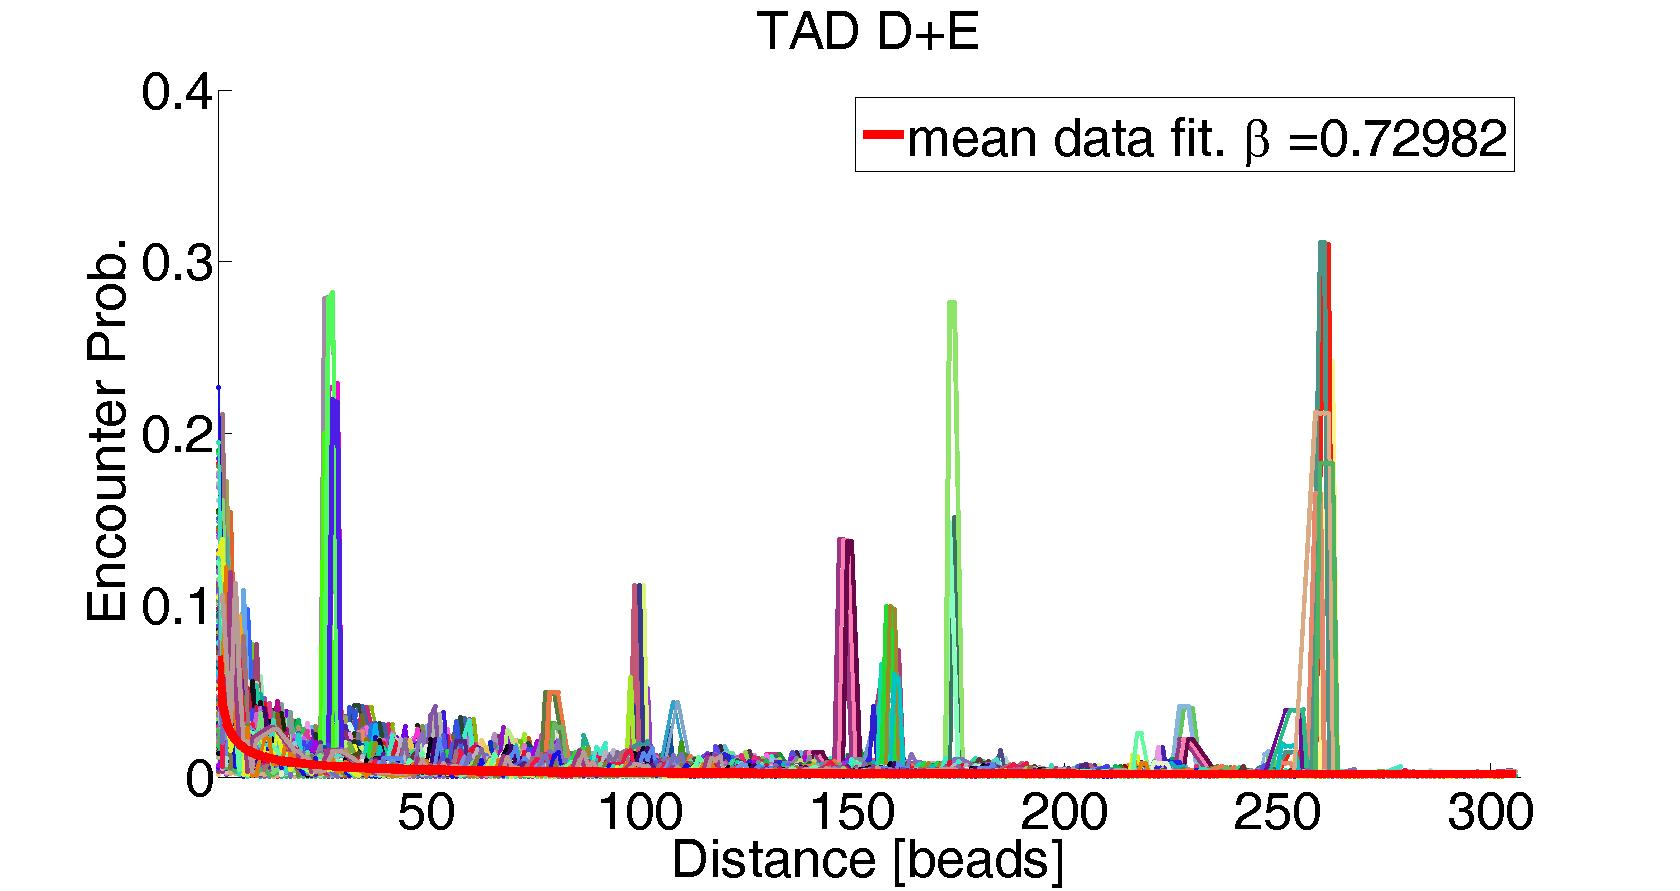
\includegraphics[scale=0.3]{meanDataFitTADDAndE}
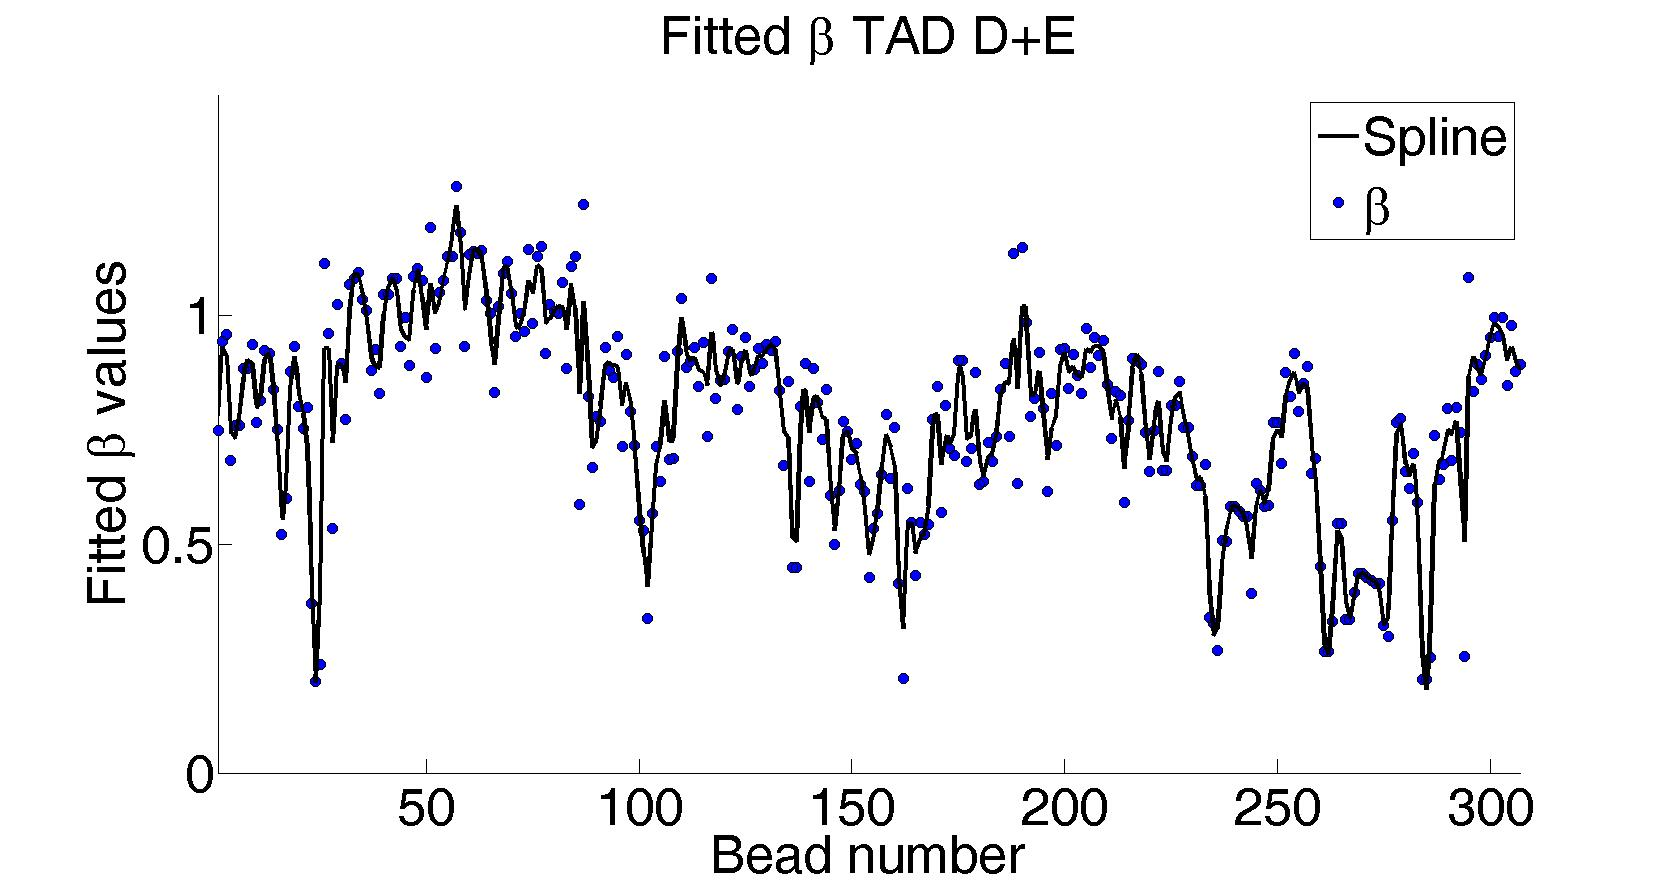
\includegraphics[scale=0.3]{fittedExpValuesWithSplineAverageTADDAndE}
\caption{}\label{figure_encounterProbabilityTADDAndE+fittedBeta}
\end{figure}
\bibliographystyle{plain}
\bibliography{randomLoopsBibliography} % the bibliography.bib
\end{document}